% Unterstützung für Links und PDF Metadaten
\documentclass[
  bibliography=totoc,     % Literatur im Inhaltsverzeichnis
  captions=tableheading,  % Tabellenüberschriften
  titlepage=firstiscover, % Titelseite ist Deckblatt
]{scrartcl}

% Paket float verbessern
\usepackage{scrhack}

% Warnung, falls nochmal kompiliert werden muss
\usepackage[aux]{rerunfilecheck}

% unverzichtbare Mathe-Befehle
\usepackage{amsmath}
% viele Mathe-Symbole
\usepackage{amssymb}
% Erweiterungen für amsmath
\usepackage{mathtools}

% Fonteinstellungen
\usepackage{fontspec}
% Latin Modern Fonts werden automatisch geladen
% Alternativ:
%\setromanfont{Libertinus Serif}
%\setsansfont{Libertinus Sans}
%\setmonofont{Libertinus Mono}
\recalctypearea % Wenn man andere Schriftarten gesetzt hat,
% sollte man das Seiten-Layout neu berechnen lassen

% deutsche Spracheinstellungen
\usepackage{polyglossia}
\setmainlanguage{german}


\usepackage[
  math-style=ISO,    % ┐
  bold-style=ISO,    % │
  sans-style=italic, % │ ISO-Standard folgen
  nabla=upright,     % │
  partial=upright,   % ┘
  warnings-off={           % ┐
    mathtools-colon,       % │ unnötige Warnungen ausschalten
    mathtools-overbracket, % │
  },                       % ┘
]{unicode-math}

% traditionelle Fonts für Mathematik
%\setmathfont{Latin Modern Math}
% Alternativ:
%\setmathfont{Libertinus Math}

%\setmathfont{XITS Math}[range={scr, bfscr}]
%\setmathfont{XITS Math}[range={cal, bfcal}, StylisticSet=1]

% Zahlen und Einheiten
\usepackage[
  locale=DE,                   % deutsche Einstellungen
  separate-uncertainty=true,   % immer Fehler mit \pm
  per-mode=symbol-or-fraction, % / in inline math, fraction in display math
]{siunitx}

% chemische Formeln
\usepackage[
  version=4,
  math-greek=default, % ┐ mit unicode-math zusammenarbeiten
  text-greek=default, % ┘
]{mhchem}

% richtige Anführungszeichen
\usepackage[autostyle]{csquotes}

% schöne Brüche im Text
\usepackage{xfrac}

% automatische Zeilenumbrüche in z.B dmath-Umgebung packet unbekannt
% \usepackage{breqn}

% Standardplatzierung für Floats einstellen
\usepackage{float}
\floatplacement{figure}{htbp}
\floatplacement{table}{htbp}


%keine Floats in anderen Sectionen
\usepackage{placeins}

\let\Oldsection\section
\renewcommand{\section}{\FloatBarrier\Oldsection}

\let\Oldsubsection\subsection
\renewcommand{\subsection}{\FloatBarrier\Oldsubsection}

\let\Oldsubsubsection\subsubsection
\renewcommand{\subsubsection}{\FloatBarrier\Oldsubsubsection}


% Seite drehen für breite Tabellen: landscape Umgebung
\usepackage{pdflscape}

% Captions schöner machen.
\usepackage[
  labelfont=bf,        % Tabelle x: Abbildung y: ist jetzt fett
  font=small,          % Schrift etwas kleiner als Dokument
  width=0.9\textwidth, % maximale Breite einer Caption schmaler
]{caption}
% subfigure, subtable, subref
\usepackage{subcaption}

% Grafiken können eingebunden werden
\usepackage{graphicx}
% größere Variation von Dateinamen möglich
\usepackage{grffile}

% schöne Tabellen
\usepackage{booktabs}

% Verbesserungen am Schriftbild
\usepackage{microtype}

% Literaturverzeichnis
\usepackage[
  backend=biber,
]{biblatex}
% Quellendatenbank
\addbibresource{lit.bib}
\addbibresource{programme.bib}

% Hyperlinks im Dokument
\usepackage[
  unicode,        % Unicode in PDF-Attributen erlauben
  pdfusetitle,    % Titel, Autoren und Datum als PDF-Attribute
  pdfcreator={},  % ┐ PDF-Attribute säubern
  pdfproducer={}, % ┘
  %colorlinks
]{hyperref}
% erweiterte Bookmarks im PDF
\usepackage{bookmark}

%erweiterte Aufzählungen
\usepackage{paralist}

% Trennung von Wörtern mit Strichen
\usepackage[shortcuts]{extdash}

\author{%
  Yascha Franz%
  \texorpdfstring{%
    \\%
    \href{mailto:yascha.franz@tu-dortmund.de}{yascha.franz@tu-dortmund.de}
  }{}%
  \texorpdfstring{\and}{, }%
  Jonah Blank%
  \texorpdfstring{%
    \\%
    \href{mailto:jonah.blank@tu-dortmund.de}{jonah.blank@tu-dortmund.de}
  }{}%
}
%\publishers{TU Dortmund – Fakultät Physik}

% Ableitungen mit \diff
\newcommand{\diff}{\mathop{}\!\mathrm{d}}

% mache . zu einem aktiven Zeichen im Mathemodus 
\mathcode`\.="8000 
% Dann kommt die Umdefinition des Dezimalpunktes 
\begingroup\lccode`~=`. 
  \lowercase{\endgroup\def~}#1{\mathrm{#1}} 
% Einstellungen hier, z.B. Fonts

\begin{document}

\section{Numerische Stabiltät}
Die beiden Funktionen
\begin{gather}
  f(x)=\left(x^3+\frac{1}{3}\right)-\left(x^3-\frac{1}{3}\right)\label{eqn:f}\\
  g(x)=\frac{\left(3+\frac{x^3}{3}\right)-\left(3-\frac{x^3}{3}\right)}{x^3}\label{eqn:g}
\end{gather}
sind beide $=2/3$.

\subsection{Untersuchung von Gleichung \eqref{eqn:f}}
\noindent Für Formel \eqref{eqn:f} lässt sich mittels der Zeilen $21-32$ in der Python-Datei bestimmen, dass der Fehler kleiner als $1\%$ ist für $-41285 \leq x \leq 41285$. Die Darstellung des relativen Fehlers ist dabei in Abbildung \ref{fig:FehlerF}, eine logarithmische Darstellung des positiven Bereichs in Abbildung \ref{fig:FehlerFlog} zu sehen.\\
Für Zahlen $|x|>165141$ ist die Gleichung numerisch $=0$.

\begin{figure}
  \centering
  \includegraphics[width=\textwidth]{build/A1_1.pdf}
  \caption{Relativer Fehler von $f(x)$ im Bereich $-41285 \leq x \leq 41285$}
  \label{fig:FehlerF}
\end{figure}

\begin{figure}
  \centering
  \includegraphics[width=\textwidth]{build/A1_12.pdf}
  \caption{Relativer Fehler von $f(x)$ im Bereich $0 \leq x \leq 41285$}
  \label{fig:FehlerFlog}
\end{figure}

\newpage

\subsection{Untersuchung von Gleichung \eqref{eqn:g}}
\noindent Mittels der Zeilen $53-58$ ist ermittelbar, daas für Werte $x>4.01269392415 \cdot 10^{-5}$ der numerische Fehler der Formel \eqref{eqn:g} kleiner als $1\%$ ist.
Für Zahlen $x<8.73291858992 \cdot 10^{-6}$ ist die Gleichung numerisch $=0$.

\begin{figure}
  \centering
  \includegraphics[width=\textwidth]{build/A1_2.pdf}
  \caption{Relativer Fehler von $g(x)$ im positiven Bereich (logarithmisch)}
  \label{fig:FehlerGlog}
\end{figure}

\newpage

\section{\texorpdfstring{$\symup{e}^-\symup{e}^+\rightarrow\gamma \gamma$}{Paarvernichtung}}
\subsection{Wirkungsquerschnitt}
Für große Werte von $\gamma=\frac{E_.e}{m_.ec^2}$ und damit $\beta\approx 1$ ist die Formel für den Wirkungsquerschnitt \eqref{eqn:WQStandard} im Bereich um $\Theta=0$ instabil, da im Nenner die Gefahr einer Auslöschung besteht. Generell ist der Nenner, da er für $\Theta\leq \frac{\pi}{2}$ immer $<1$ ist, eine Gefahr für Instabilität, weil so durch eine kleine Zahl geteilt wird.\\
Beheben lässt sich dies durch Umformungen mit den Beziehungen

\begin{gather}
  1-\beta^2=\frac{1}{\gamma^2}\nonumber\\
  1=\sin^2(\Theta)+\cos^2(\Theta)\nonumber
\end{gather}
zu Formel \eqref{eqn:WQModifiziert}.

\begin{align}
    \frac{\mathrm{d}\sigma}{\mathrm{d}\Omega} &= \frac{\alpha^2}{s} \left(\frac{2+\sin(\Theta)}{1-\beta^2 \cos(\Theta)}\right)^2\label{eqn:WQStandard}\\
&= \frac{\alpha^2}{s}\frac{2+\sin^2(\Theta)}{\frac{1}{\gamma^2}\cos^2(\Theta)+\sin^2(\Theta)}\label{eqn:WQModifiziert}
\end{align}
Hierbei ist

\begin{gather}
  s=(2E_\text{e})^2 \;\;(E_\text{e} \text{ ist die Energie der Teilchen im Schwerpunktssystem})\text{.}\nonumber
\end{gather}

\noindent In den Abbildungen \ref{fig:t0} bis \ref{fig:tpi}, die im Code über die Zeilen $74$-$122$ erzeugt werden, sind die Bereiche um $\Theta=0$, $\Theta=\frac{\pi}{2}$ und $\Theta=\pi$ zu sehen.
Daran lassen sich kaum Unterschiede ablesen, auch weil der Nenner nach wie vor sehr klein ist. Trägt man allerdings in Abbildung \ref{fig:Abweichung} die Differenz zwischen den beiden Versionen gegen $\Theta$ auf, lässt sich erkennen, das diese sich für Werte um $\Theta=0$ bzw. $2\pi$ deutlich unterscheiden.

\begin{figure}
  \centering
  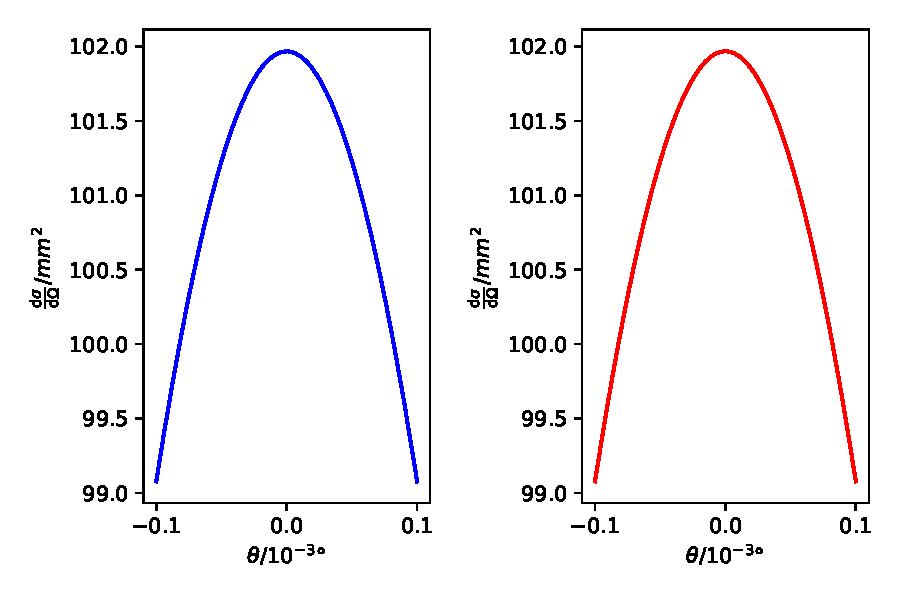
\includegraphics[width=\textwidth]{build/plot1.pdf}
  \caption{\eqref{eqn:WQStandard} und \eqref{eqn:WQModifiziert} um $\Theta = 0$}
  \label{fig:t0}
\end{figure}

\begin{figure}
  \centering
  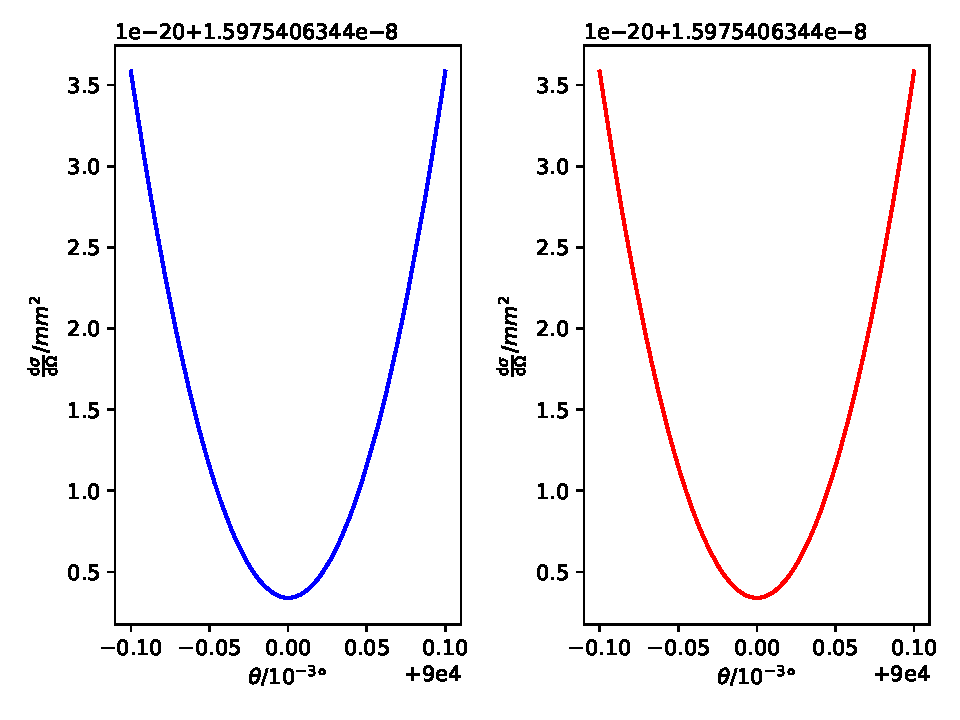
\includegraphics[width=\textwidth]{build/plot2.pdf}
  \caption{\eqref{eqn:WQStandard} und \eqref{eqn:WQModifiziert} um $\Theta = \frac{\pi}{2}$}
  \label{fig:tpi2}
\end{figure}

\begin{figure}
  \centering
  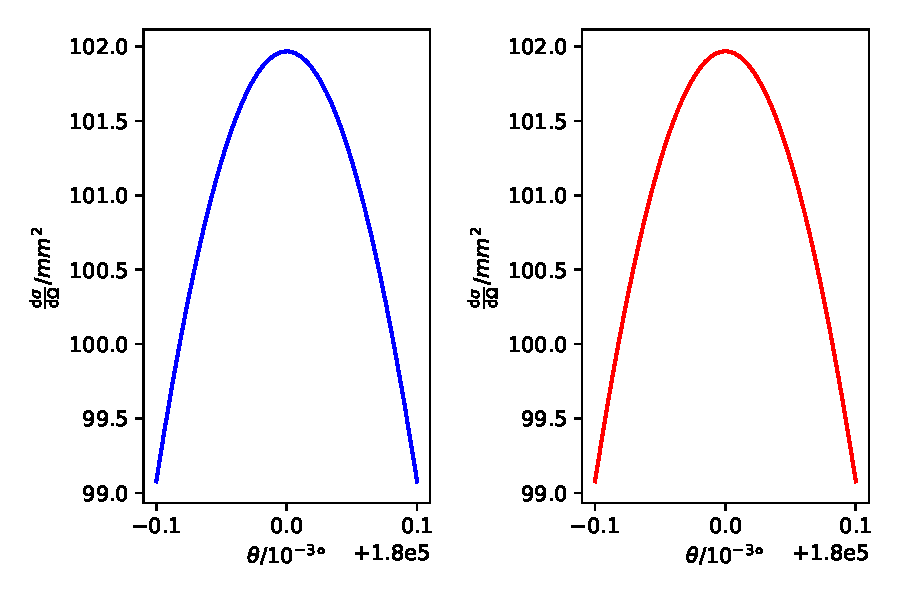
\includegraphics[width=\textwidth]{build/plot3.pdf}
  \caption{\eqref{eqn:WQStandard} und \eqref{eqn:WQModifiziert} um $\Theta = \pi$}
  \label{fig:tpi}
\end{figure}

\begin{figure}
  \centering
  \includegraphics[width=\textwidth]{build/Differenz.pdf}
  \caption{Die Differenz von \eqref{eqn:WQStandard} und \eqref{eqn:WQModifiziert} im Bereich $0 \leq \Theta \leq 2\pi$}
  \label{fig:Abweichung}
\end{figure}

\newpage

\subsection{Konditionszahl}
Aus der Beziehung für die Konditionszahl
\begin{equation}
  K(x):=\left|x\frac{f'(x)}{f(x)}\right|
\end{equation}
ergibt sich die Formel \eqref{eqn:K} und damit den Graphen \ref{fig:kondition}.
\begin{equation}
  K(\Theta)= \Theta  \left|\frac{2\sin(\Theta)\cos(\Theta)\left(1-3\beta^2\right)}{\left(2+\sin^2(\Theta)\right)\left(1-\beta^2\cos^2(\Theta)\right)}\right| \label{eqn:K}
\end{equation}

\begin{figure}
  \centering
  \includegraphics{build/kondition.pdf}
  \caption{Konditionszahl in Abhängigkeit des Winkels}
  \label{fig:kondition}
\end{figure}
\noindent Aus dem Plot \ref{fig:kondition}, der in den Zeilen $140$-$146$ erzeugt wird, ist erkennbar, dass das Problem im Bereich um $180\si{\degree}$ schlecht konditioniert ist.
Überall sonst ist es sehr gut konditioniert.

\end{document}



%☺¶
